%%%%%%%%%%%%%%%%%%%%%%%%%%%%%%%%%%%%%%%%%%%%%%%%%%
%
%  New template code for TAMU Theses and Dissertations starting Fall 2012.  
%  For more info about this template or the 
%  TAMU LaTeX User's Group, see http://www.howdy.me/.
%
%  Author: Wendy Lynn Turner 
%	 Version 1.0 
%  Last updated 8/5/2012
%
%%%%%%%%%%%%%%%%%%%%%%%%%%%%%%%%%%%%%%%%%%%%%%%%%%%
%%%%%%%%%%%%%%%%%%%%%%%%%%%%%%%%%%%%%%%%%%%%%%%%%%%%%%%%%%%%%%%%%%%%%%
%%                           SECTION IV
%%%%%%%%%%%%%%%%%%%%%%%%%%%%%%%%%%%%%%%%%%%%%%%%%%%%%%%%%%%%%%%%%%%%%

\chapter{\uppercase{Implementation}}

The main goal of Seismic Data Analytics SDK is to develop a scalable and distributed software development tool to enable scalable computation and analytics of seismic volume datasets. This chapter will present the software architecture and the main functionalities of SDK, as well as some utilities we have built for user to deploy their applications on this big data platform.

\section{Architecture}

Seismic Data Analytics SDK is built upon Apache Hadoop and Spark. Figure \ref{sdk_swstack} shows the software stack of a workable seismic data analytics platform. As shown in this diagram, the gray part is the OS layer, the elements with green color stands for the infrastructure layer of this big data platform, and on top of that, the components with blue color is the SDK. At the bottom of infrastructure layer, there is Hadoop Distributed File System (HDFS) that stores the big seismic data files by utilizing the large number of local disks. The Cassandra as a NoSQL database is also used to store  seismic data, intermediate results and meta data. YARN and Mesos are used for resources management. Apache Spark is the data distribution and parallel execution engine based on the innovative idea of Resilient Distributed DataSets (RDD) concept. MLLib is included in the Spark as the machine learning package to enable machine learning based data analytics algorithms. OpenCV is the widely used image processing package that is used to provide image processing capability. Breeze is the numerical processing package including linear algebra, signal processing, statistics, and other numerical computation and optimizations written in Scala. We have developed the seismic data RDD on top of Spark as the base distributed seismic datasets to enable parallel operations and machine learning algorithms. Geophysicists and data scientists can use the Seismic Data Analytics SDK to develop their own algorithms and leverage the capability of Apache Spark provides, as well as image processing, numerical computation, and deep learning packages.

\begin{figure}[h]
\centering
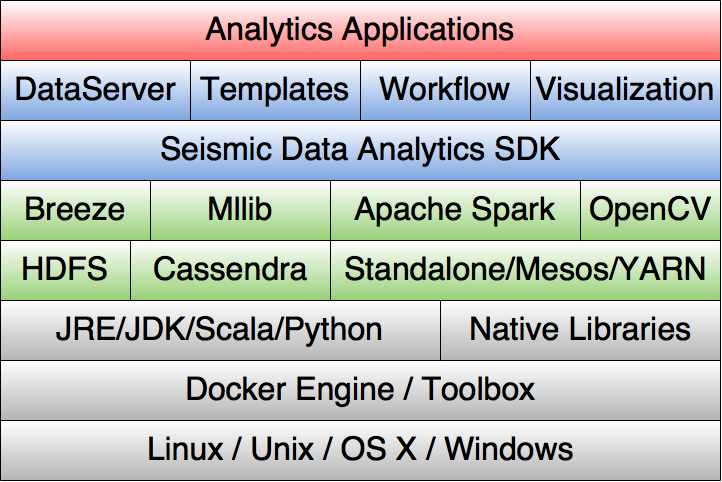
\includegraphics[scale=0.4]{figures/sdk_swstack.png}
\caption{Software Stack of Seismic Data Analytics Platform}
\label{sdk_swstack}
\end{figure}

Figure \ref{sdk_framework} simplifies the development efforts for scalable and distributed computing and analytics of seismic datasets. It is built on top of the Apache Hadoop and Spark. The Hadoop provides a distributed file system(HDFS) and resource management system (YARN and Mesos), while Spark provides a high-level distributed data representation via Resilient Data Sets (RDD) and a data-parallelism execution engine. Seismic Data Analytics SDK provides configurable data distribution fashions for seismic volume data, as well as a configurable parallel execution interface to simplify the parallel programming efforts. Based on the functionality of SDK, we developed two useful utilities, parallel templates and data server, to facilitate SDK for users to easily deploy their applications. Moreover, since Hadoop and Spark provide faults tolerance and task scheduling utilities, the toolkit inherits from them to provide fault tolerance and dynamic task scheduling for better reliability and task management.

\begin{figure}[h]
\centering
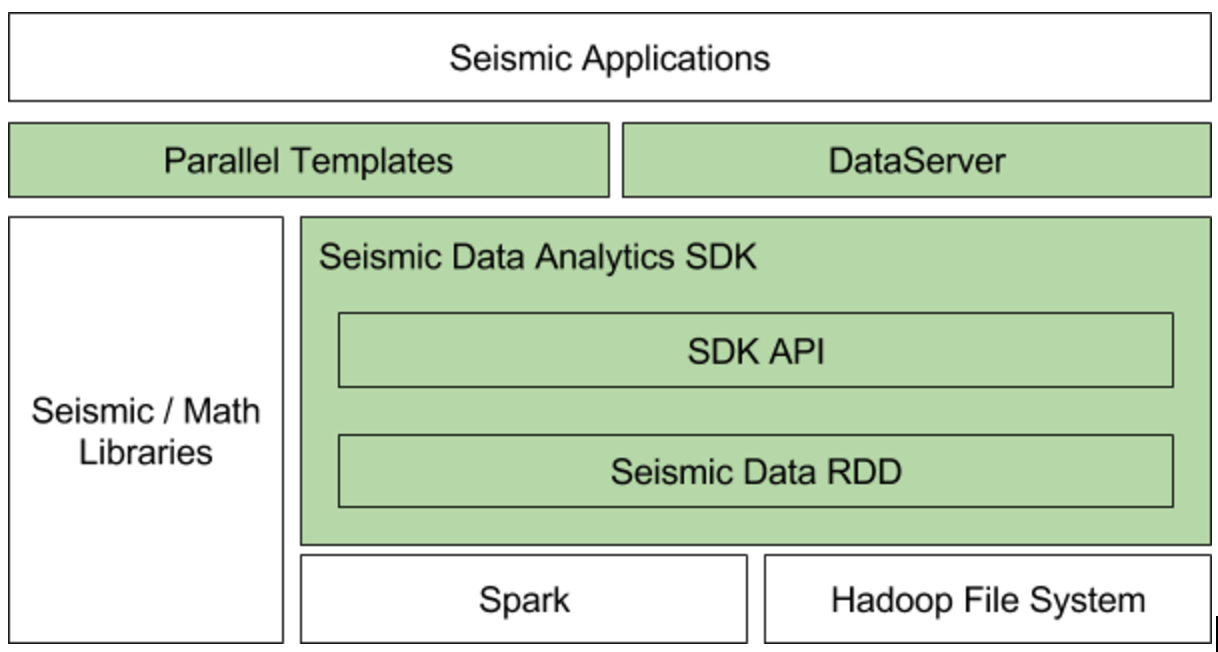
\includegraphics[scale=0.4]{figures/sdk_framework.png}
\caption{Framework of Seismic Data Analytics SDK}
\label{sdk_framework}
\end{figure}


\section{Interfaces and Functionalities}

\subsection{Seismic Volume Data Loading,  Distribution and Saving}

\subsection{Volume Data Accessing}

\subsection{Volume Data 3D Transposing}

\subsection{Distribution Aggregation}

\subsection{Distribution Overlapping}

\subsection{User Defined Function Mapping}


\section{Application Utilities}

\subsection{Parallel Templates}

\subsection{Data Server and Remote Web Visualization}

\subsection{Web-based Workflow Platform}

